% Title: gl2ps_renderer figure
% Creator: GL2PS 1.4.2, (C) 1999-2020 C. Geuzaine
% For: Octave
% CreationDate: Tue Oct 26 16:41:12 2021
\setlength{\unitlength}{1pt}
\begin{picture}(0,0)
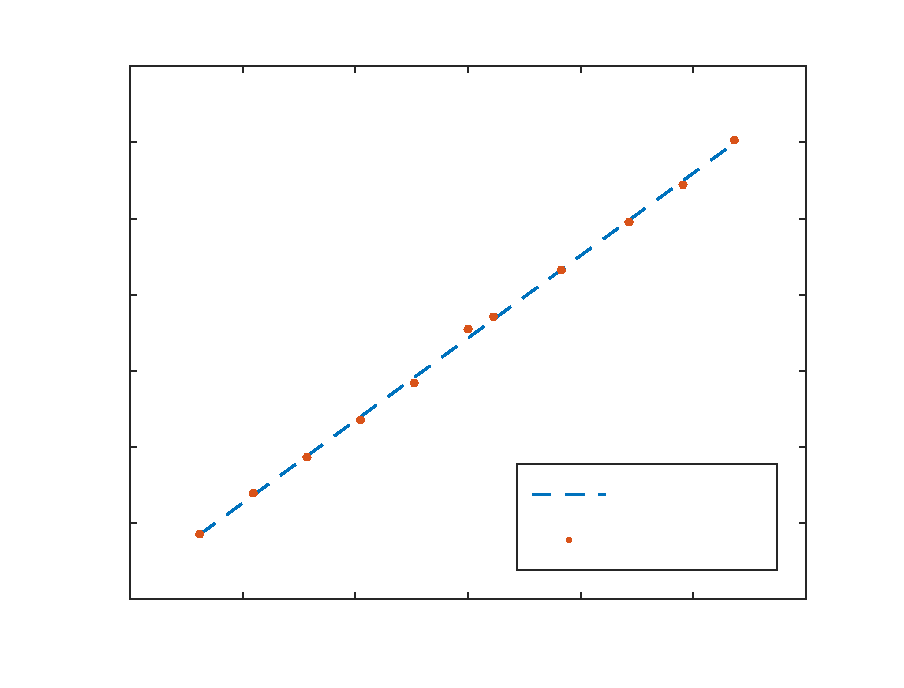
\includegraphics[scale=1]{linreg_ext-inc}
\end{picture}%
\begin{picture}(418,314)(0,0)
\fontsize{10}{0}\selectfont\put(54.4343,27.0024){\makebox(0,0)[t]{\textcolor[rgb]{0.15,0.15,0.15}{{-6}}}}
\fontsize{10}{0}\selectfont\put(108.52,27.0024){\makebox(0,0)[t]{\textcolor[rgb]{0.15,0.15,0.15}{{-4}}}}
\fontsize{10}{0}\selectfont\put(162.605,27.0024){\makebox(0,0)[t]{\textcolor[rgb]{0.15,0.15,0.15}{{-2}}}}
\fontsize{10}{0}\selectfont\put(216.69,27.0024){\makebox(0,0)[t]{\textcolor[rgb]{0.15,0.15,0.15}{{0}}}}
\fontsize{10}{0}\selectfont\put(270.776,27.0024){\makebox(0,0)[t]{\textcolor[rgb]{0.15,0.15,0.15}{{2}}}}
\fontsize{10}{0}\selectfont\put(324.861,27.0024){\makebox(0,0)[t]{\textcolor[rgb]{0.15,0.15,0.15}{{4}}}}
\fontsize{10}{0}\selectfont\put(378.946,27.0024){\makebox(0,0)[t]{\textcolor[rgb]{0.15,0.15,0.15}{{6}}}}
\fontsize{10}{0}\selectfont\put(49.4418,34.5008){\makebox(0,0)[r]{\textcolor[rgb]{0.15,0.15,0.15}{{-2}}}}
\fontsize{10}{0}\selectfont\put(49.4418,71.0645){\makebox(0,0)[r]{\textcolor[rgb]{0.15,0.15,0.15}{{-1.5}}}}
\fontsize{10}{0}\selectfont\put(49.4418,107.628){\makebox(0,0)[r]{\textcolor[rgb]{0.15,0.15,0.15}{{-1}}}}
\fontsize{10}{0}\selectfont\put(49.4418,144.192){\makebox(0,0)[r]{\textcolor[rgb]{0.15,0.15,0.15}{{-0.5}}}}
\fontsize{10}{0}\selectfont\put(49.4418,180.756){\makebox(0,0)[r]{\textcolor[rgb]{0.15,0.15,0.15}{{0}}}}
\fontsize{10}{0}\selectfont\put(49.4418,217.319){\makebox(0,0)[r]{\textcolor[rgb]{0.15,0.15,0.15}{{0.5}}}}
\fontsize{10}{0}\selectfont\put(49.4418,253.883){\makebox(0,0)[r]{\textcolor[rgb]{0.15,0.15,0.15}{{1}}}}
\fontsize{10}{0}\selectfont\put(49.4418,290.447){\makebox(0,0)[r]{\textcolor[rgb]{0.15,0.15,0.15}{{1.5}}}}
\fontsize{11}{0}\selectfont\put(26.4418,162.474){\rotatebox{90}{\makebox(0,0)[b]{\textcolor[rgb]{0.15,0.15,0.15}{{Tensão do extensómetro (V)}}}}}
\fontsize{11}{0}\selectfont\put(216.69,14.0024){\makebox(0,0)[t]{\textcolor[rgb]{0.15,0.15,0.15}{{Deflexão da barra (deg)}}}}
\fontsize{9}{0}\selectfont\put(289.78,84.9481){\makebox(0,0)[l]{\textcolor[rgb]{0,0,0}{{Regressão linear}}}}
\fontsize{9}{0}\selectfont\put(289.78,63.0759){\makebox(0,0)[l]{\textcolor[rgb]{0,0,0}{{Dados recolhidos}}}}
\end{picture}
